\section{Resultados}
\label{resultados}

\subsection{Redução da Distância (Q1)}
\label{ssec:q1}

Para avaliar a eficiência das estratégias de coleta no Modelo 1, foram analisados 10.000 pedidos reais do conjunto \textit{train} do Instacart, utilizando a grade $9 \times 15$. As estratégias de ordem do carrinho, ordem aleatória e vizinho mais próximo foram avaliadas nos 10.000 pedidos, enquanto o ótimo exato foi calculado para os 9.222 pedidos com até 15 \textit{aisles} distintos. Para a ordem aleatória, foram realizados cinco sorteios por pedido. As distâncias médias obtidas foram de 74,37 passos para a ordem do carrinho, 75,05 para a aleatória e 43,82 para o vizinho mais próximo, conforme a Tabela~\ref{tab:custos}. Os 10.000 pedidos correspondem aos primeiros identificadores ordenados do recorte, não a uma amostra aleatória.

\begin{table}[!ht]
\caption{Custos médios, em passos, das estratégias de coleta na grade $9 \times 15$, calculados sobre 10.000 pedidos do conjunto \textit{train} do Instacart, durante a avaliação experimental do projeto.}
\label{tab:custos}
\centering
\small
\begin{tabular}{lrr}
\hline
\textbf{Estratégia} & \textbf{Distância média} & \textbf{Pedidos} \\
 & \textbf{(passos)} & \textbf{avaliados} \\ \hline
Ordem do carrinho & 74,37 & 10.000 \\
Ordem aleatória & 75,05 & 10.000 \\
Vizinho mais próximo & 43,82 & 10.000 \\
Ótimo exato (Held-Karp) & 39,10 & 9.222 \\ \hline
\end{tabular}
\end{table}

Em relação à ordem do carrinho, o vizinho mais próximo reduziu a distância média em 41,08\%, produzindo percursos menores em 7.626 pedidos (76,26\%), equivalentes em 2.219 (22,19\%) e maiores em 155 (1,55\%). Nos 9.222 pedidos com solução ótima, apresentou \textit{gap} médio de 6,71\% e alcançou o ótimo em 49,83\% dos casos. A média de 39,10 passos do Held-Karp refere-se somente a esse subconjunto.

\subsection{Efeito do Número de Pontos de Coleta Obrigatórios (Q2)}
\label{ssec:q2}

A quantidade de \textit{aisles} distintos por pedido influencia diretamente o custo das rotas e a diferença de desempenho entre as estratégias. Nos 10.000 pedidos avaliados, 1.413 possuíam apenas um ou dois pontos obrigatórios, casos em que todas as estratégias produziram distâncias equivalentes e ótimas, independentemente da ordem de visita.

A partir de três \textit{aisles}, as diferenças tornam-se mais evidentes. Para pedidos com três pontos obrigatórios, o vizinho mais próximo apresentou menor custo que a ordem do carrinho em 38,10\% dos casos. Com nove \textit{aisles}, essa proporção alcançou 99,84\%, demonstrando que a escolha da sequência de coleta ganha importância conforme aumenta o número de pontos a visitar.

\begin{figure}[!ht]
\centering
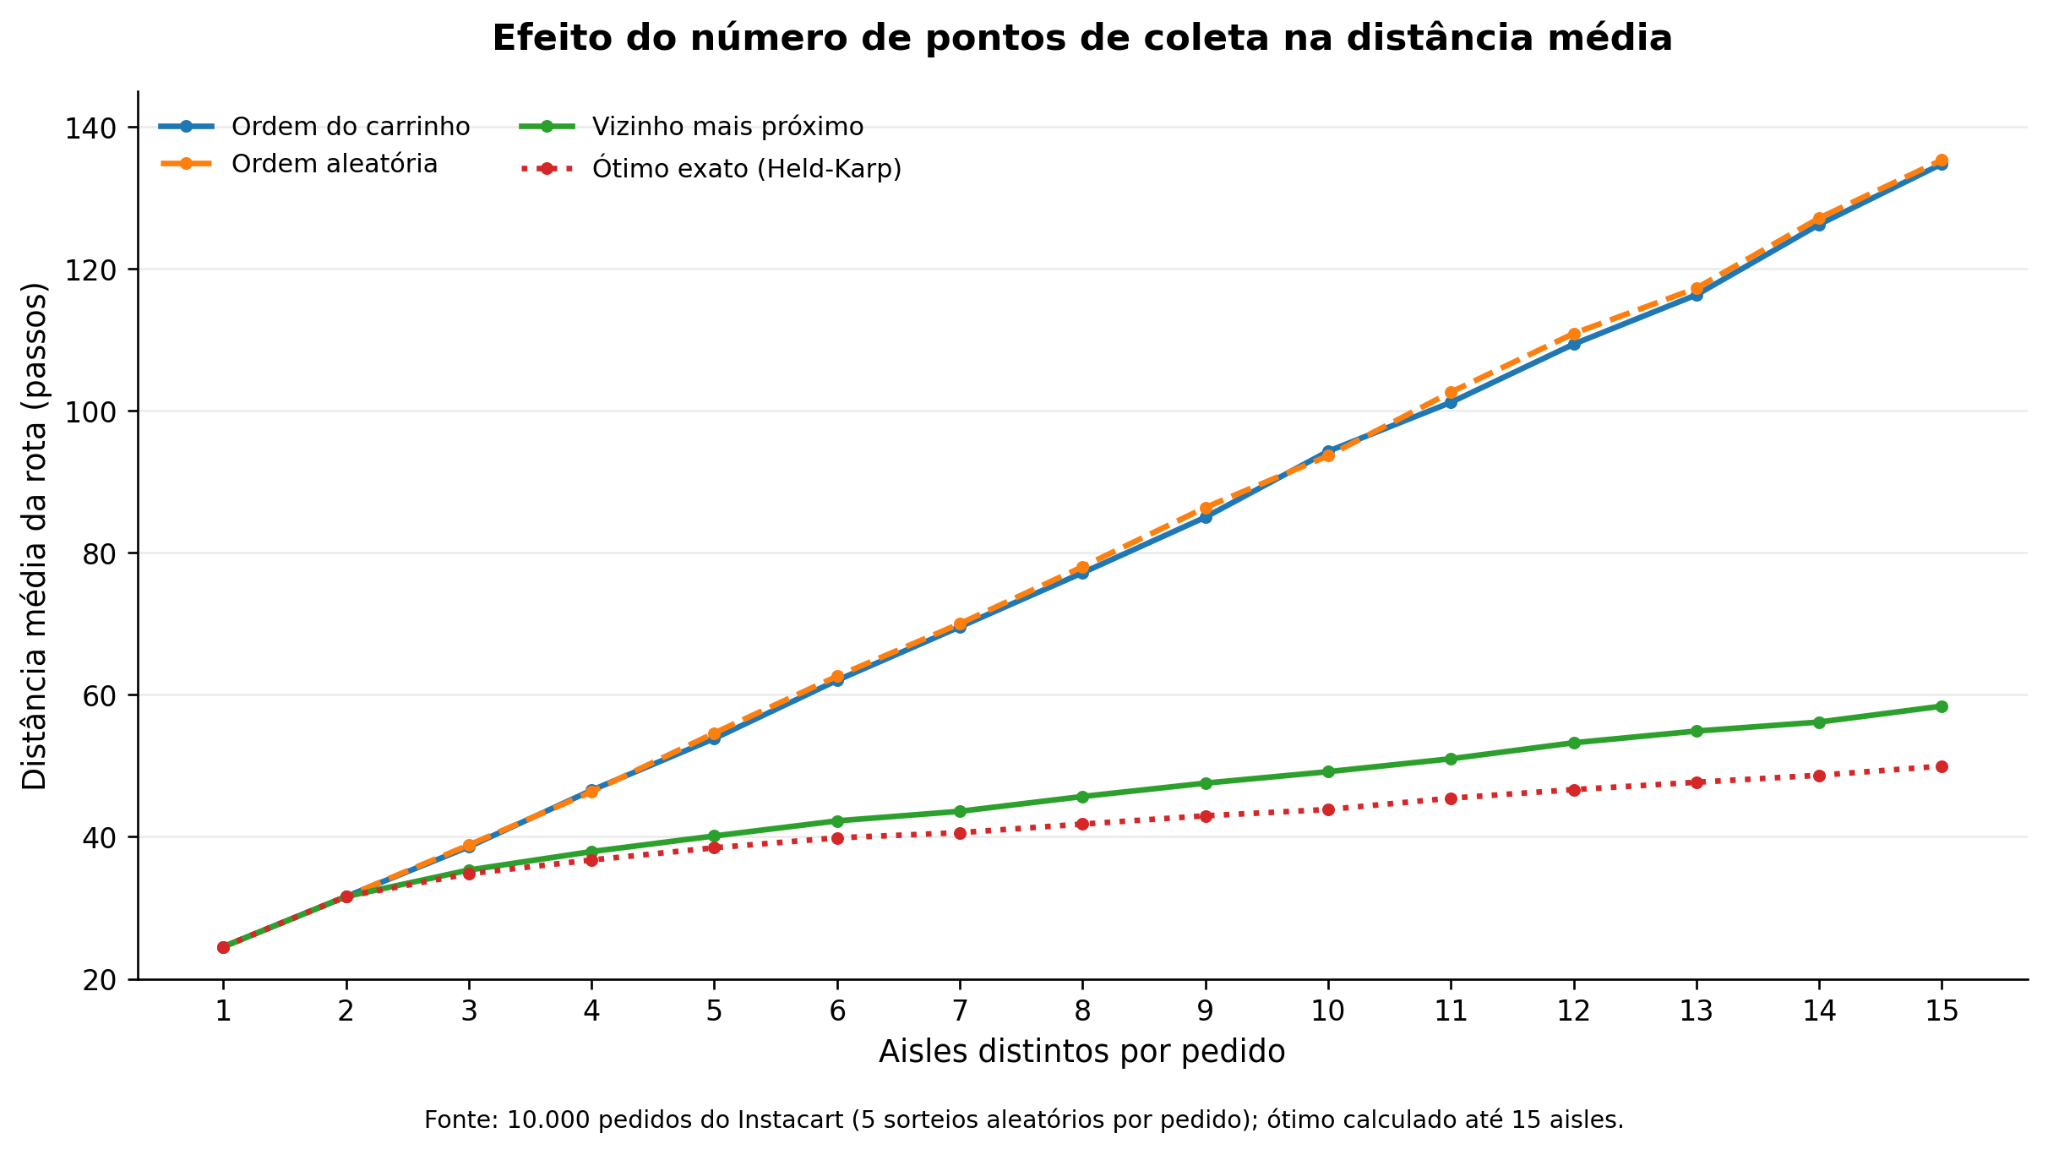
\includegraphics[width=\columnwidth]{figs/custo_por_aisles.png}
\caption{Distância média das rotas, em passos, por número de \textit{aisles} distintos, considerando os 10.000 pedidos avaliados no Modelo 1. São comparadas a ordem do carrinho, a ordem aleatória, o vizinho mais próximo e a solução ótima exata, calculada para pedidos com até 15 \textit{aisles}.}
\label{fig:custo_aisles}
\end{figure}

Conforme a Figura~\ref{fig:custo_aisles}, entre três e quinze \textit{aisles}, a distância média da ordem do carrinho aumentou de 38,60 para 134,81 passos, enquanto a do vizinho mais próximo passou de 35,32 para 58,42 passos. Nesse intervalo, a solução ótima apresentou médias de 34,81 a 49,96 passos.

Nos 778 pedidos com mais de quinze \textit{aisles}, para os quais não foi calculada a solução ótima, o vizinho mais próximo manteve menor distância média (65,31 passos) que a ordem do carrinho (166,32 passos). Os resultados indicam que o benefício do roteamento heurístico se torna mais expressivo em pedidos com maior quantidade de pontos de coleta, embora a estratégia não garanta o percurso ótimo.

\subsection{Layout Guiado por Coocorrência (Q3)}
\label{ssec:q3}

Nos 26.242 pedidos de teste, o layout reorganizado reduziu a distância média da ordem do carrinho de 74,39 para 53,27 passos (28,39\%) e a do vizinho mais próximo de 43,86 para 36,09 passos (17,72\%). Como esse conjunto de teste não coincide com o recorte de 10.000 pedidos do Modelo 1, as médias no layout original diferem ligeiramente das apresentadas na Tabela~\ref{tab:custos}. A Figura~\ref{fig:layouts} apresenta o layout original e o reorganizado por coocorrência, obtido após 30 trocas de posição entre \textit{aisles}, mantendo o caixa fixo.

\begin{figure*}[!t]
\centering
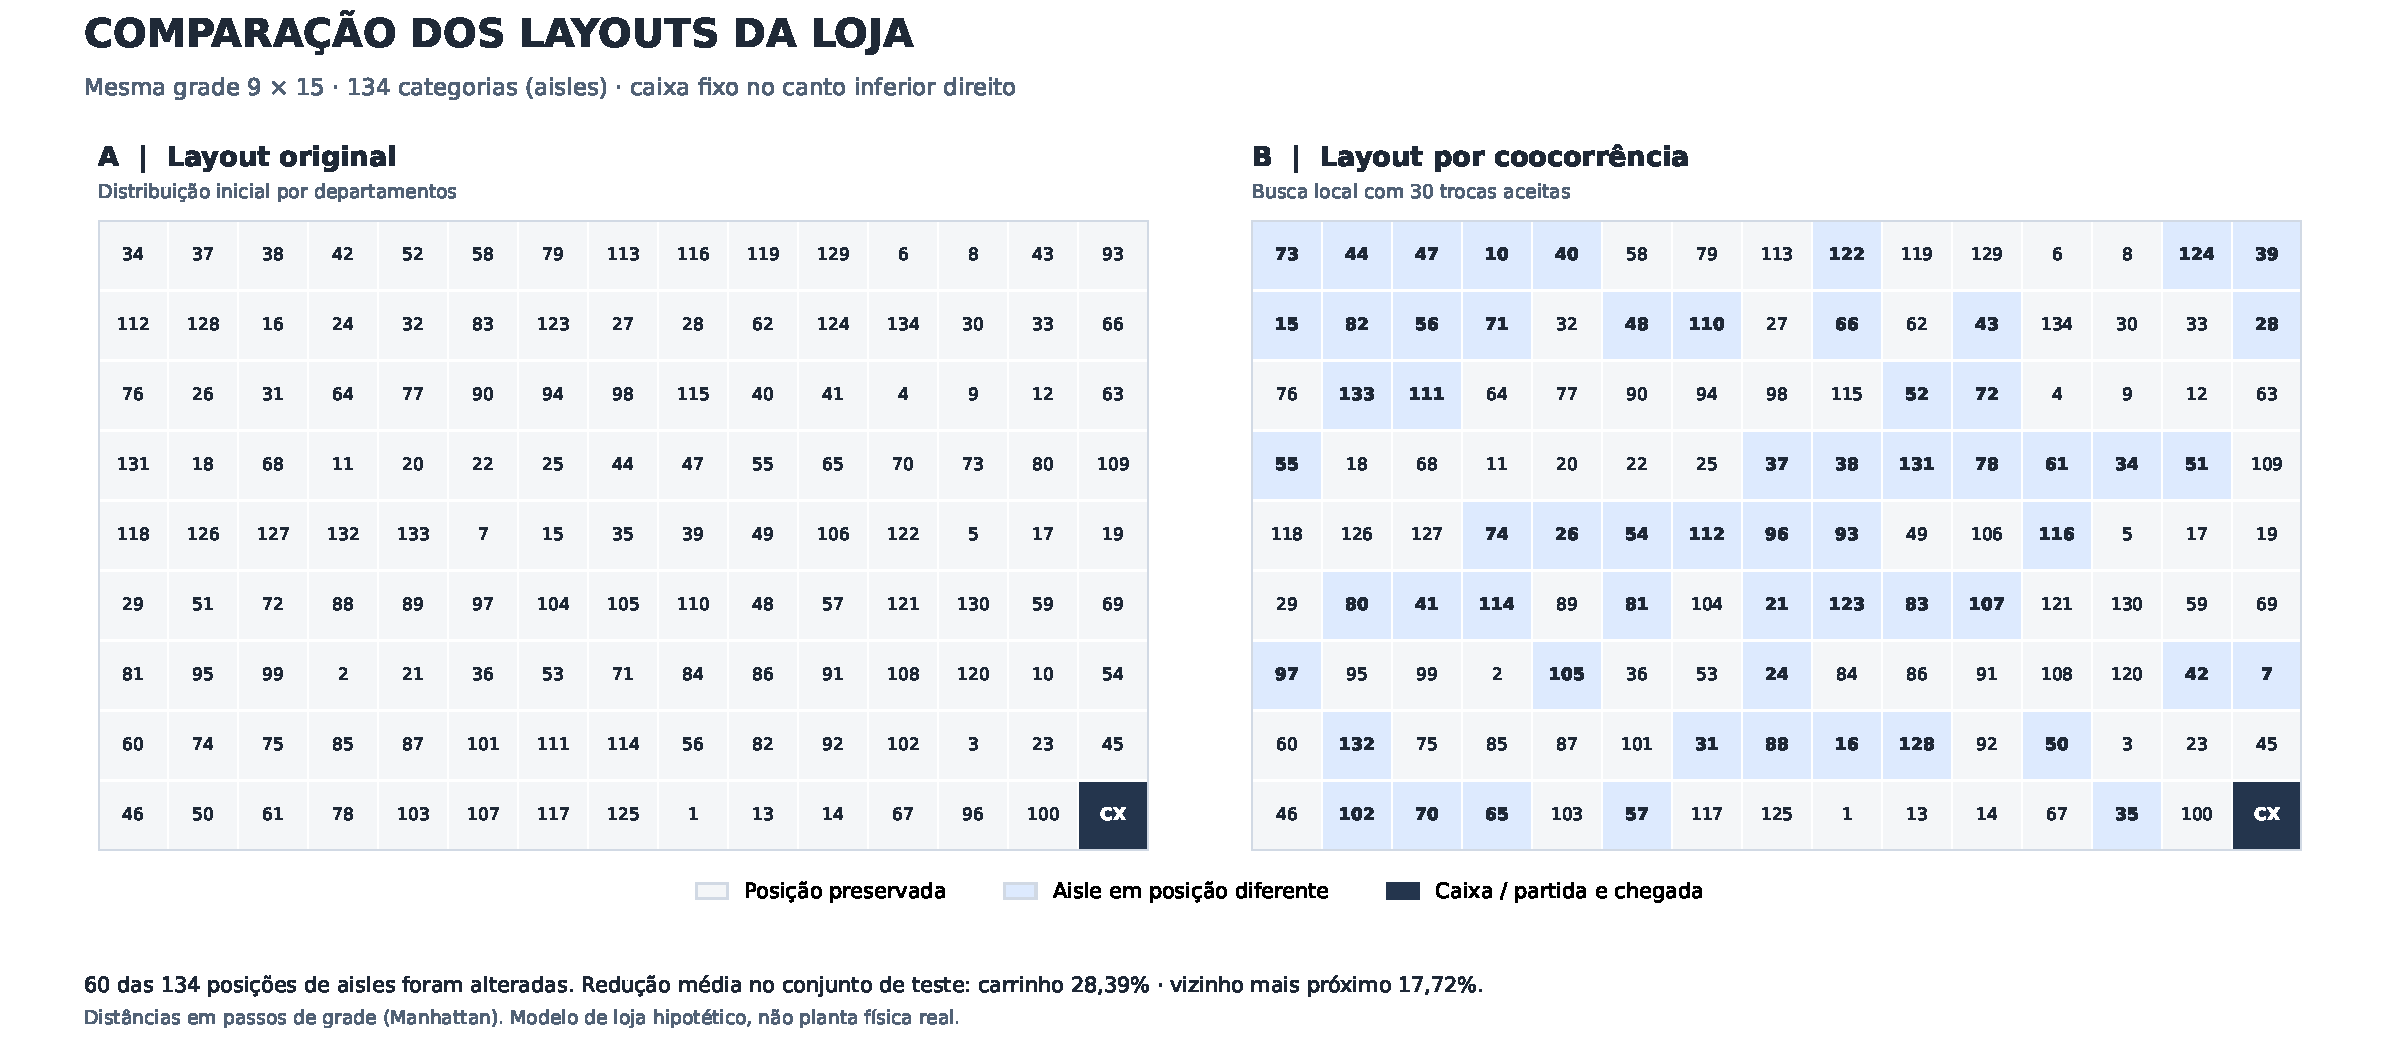
\includegraphics[width=0.86\textwidth]{figs/comparacao_layouts.pdf}
\caption{Comparação dos layouts original e otimizado por coocorrência, em uma grade $9 \times 15$, após 30 trocas de posição entre \textit{aisles}. A avaliação das distâncias considera 26.242 pedidos de teste do Instacart.}
\label{fig:layouts}
\end{figure*}

A otimização do layout utilizou 8.466 associações ponderadas pela similaridade de Jaccard. Após 30 trocas de posições, a função objetivo diminuiu de 1.681,92 para 1.318,52, uma redução de 21,61\%. Essa medida representa a redução das distâncias ponderadas entre categorias associadas, não diretamente o custo das rotas. A Tabela~\ref{tab:layouts} compara os resultados individuais dos layouts original e otimizado nos 26.242 pedidos de teste.

\begin{table}[!ht]
\caption{Comparação individual das distâncias entre os layouts original e otimizado por coocorrência, considerando 26.242 pedidos de teste do Instacart.}
\label{tab:layouts}
\centering
\small
\begin{tabular}{lrrr}
\hline
\textbf{Estratégia} & \textbf{Menor} & \textbf{Equivalente} & \textbf{Maior} \\ \hline
Ordem do & 21.932 & 2.472 & 1.838 \\
\quad carrinho & (83,58\%) & (9,42\%) & (7,00\%) \\
Vizinho mais & 19.153 & 3.507 & 3.582 \\
\quad próximo & (72,99\%) & (13,36\%) & (13,65\%) \\ \hline
\end{tabular}
\end{table}

O layout otimizado apresentou percursos menores na maioria dos pedidos para ambas as estratégias, embora também tenham ocorrido empates e aumentos de distância. Dessa forma, os resultados indicam que a reorganização orientada pela coocorrência favoreceu a eficiência média da coleta no ambiente simulado, sem garantir melhorias individuais para todos os pedidos.

\subsection{Impacto Operacional da Organização Espacial (Q4)}
\label{ssec:q4}

Os dois layouts preservam a grade $9 \times 15$ e a posição do caixa, alterando apenas a distribuição dos \textit{aisles}. Dessa forma, a comparação avalia os efeitos da reorganização espacial, sem modificar a conectividade da loja hipotética.

Para estimar o impacto operacional dessa reorganização, foram utilizadas as distâncias médias obtidas nos 26.242 pedidos de teste. Consideraram-se, como hipóteses, 1,5 metro por passo, velocidade de deslocamento de 1,2~m/s, 20 segundos de separação por item, 120 segundos fixos por pedido e sete horas efetivas de trabalho por turno, para um funcionário (Tabela~\ref{tab:operacional}).

\begin{table}[!ht]
\caption{Tempo médio estimado de coleta e capacidade por turno nos layouts original e otimizado, considerando os 26.242 pedidos de teste do Instacart e as hipóteses operacionais adotadas.}
\label{tab:operacional}
\centering
\small
\begin{tabular}{@{}p{0.30\columnwidth}lrr@{}}
\hline
\textbf{Estratégia} & \textbf{Layout} & \textbf{Min/} & \textbf{Pedidos/} \\
 & & \textbf{pedido} & \textbf{turno} \\ \hline
Ordem do carrinho & Original & 7,06 & 59 \\
Ordem do carrinho & Coocorrência & 6,62 & 63 \\
Vizinho mais próximo & Original & 6,42 & 65 \\
Vizinho mais próximo & Coocorrência & 6,26 & 67 \\ \hline
\end{tabular}
\end{table}

A reorganização elevou a capacidade estimada de 59 para 63 pedidos por turno na ordem do carrinho e de 65 para 67 no vizinho mais próximo. Embora a redução dos deslocamentos contribua para diminuir o tempo total, atividades como separação, conferência e preparação dos pedidos permanecem necessárias.

\subsection{Discussão}
\label{ssec:discussao}

Os resultados indicam que tanto a estratégia de roteamento quanto a organização espacial das categorias influenciam a distância percorrida. No Modelo 1, a ordem do carrinho (74,37 passos) apresentou desempenho praticamente igual ao da ordem aleatória (75,05 passos). Como a sequência em que o cliente adiciona os produtos não segue a disposição física da loja, utilizá-la como roteiro equivale, na prática, a coletar sem critério, o que reforça a relevância do problema estudado.

O vizinho mais próximo reduziu a distância média em 41,08\% em relação à ordem do carrinho e ficou, em média, 6,71\% acima do ótimo exato. Esse comportamento é coerente com a literatura: embora a heurística não ofereça garantia de desempenho no pior caso \citep{rosenkrantz1977,hougardy2015}, costuma produzir rotas próximas do ótimo em instâncias típicas \citep{johnson1997}. A vantagem cresce com o número de pontos de coleta, pois pedidos maiores admitem mais ordens de visita e, portanto, mais oportunidades de deslocamentos desnecessários quando não há critério.

No Modelo 2, a reorganização por coocorrência reduziu as distâncias médias de ambas as estratégias. A função objetivo aproxima categorias adquiridas em conjunto, mas, ao deslocar categorias frequentes para junto de suas associadas, a reorganização também as aproximou do caixa: frutas frescas passaram de 18 para 9 passos do caixa, vegetais frescos de 16 para 8 e frutas e vegetais embalados de 15 para 9. Assim, a redução observada reflete dois efeitos da mesma reorganização: a proximidade entre categorias associadas e a proximidade de categorias frequentes ao ponto de partida das rotas. Ambos resultam do layout guiado pelo grafo de coocorrência, ainda que o segundo não seja um objetivo explícito da função objetivo; a redução obtida permanece, portanto, um resultado do layout proposto, mas este estudo não separa a contribuição de cada efeito.

No aspecto operacional, a redução de distância se traduz em ganhos proporcionalmente menores de tempo, pois a separação dos itens, a conferência e a preparação dos pedidos independem do trajeto.

\begin{figure}[!ht]
\centering
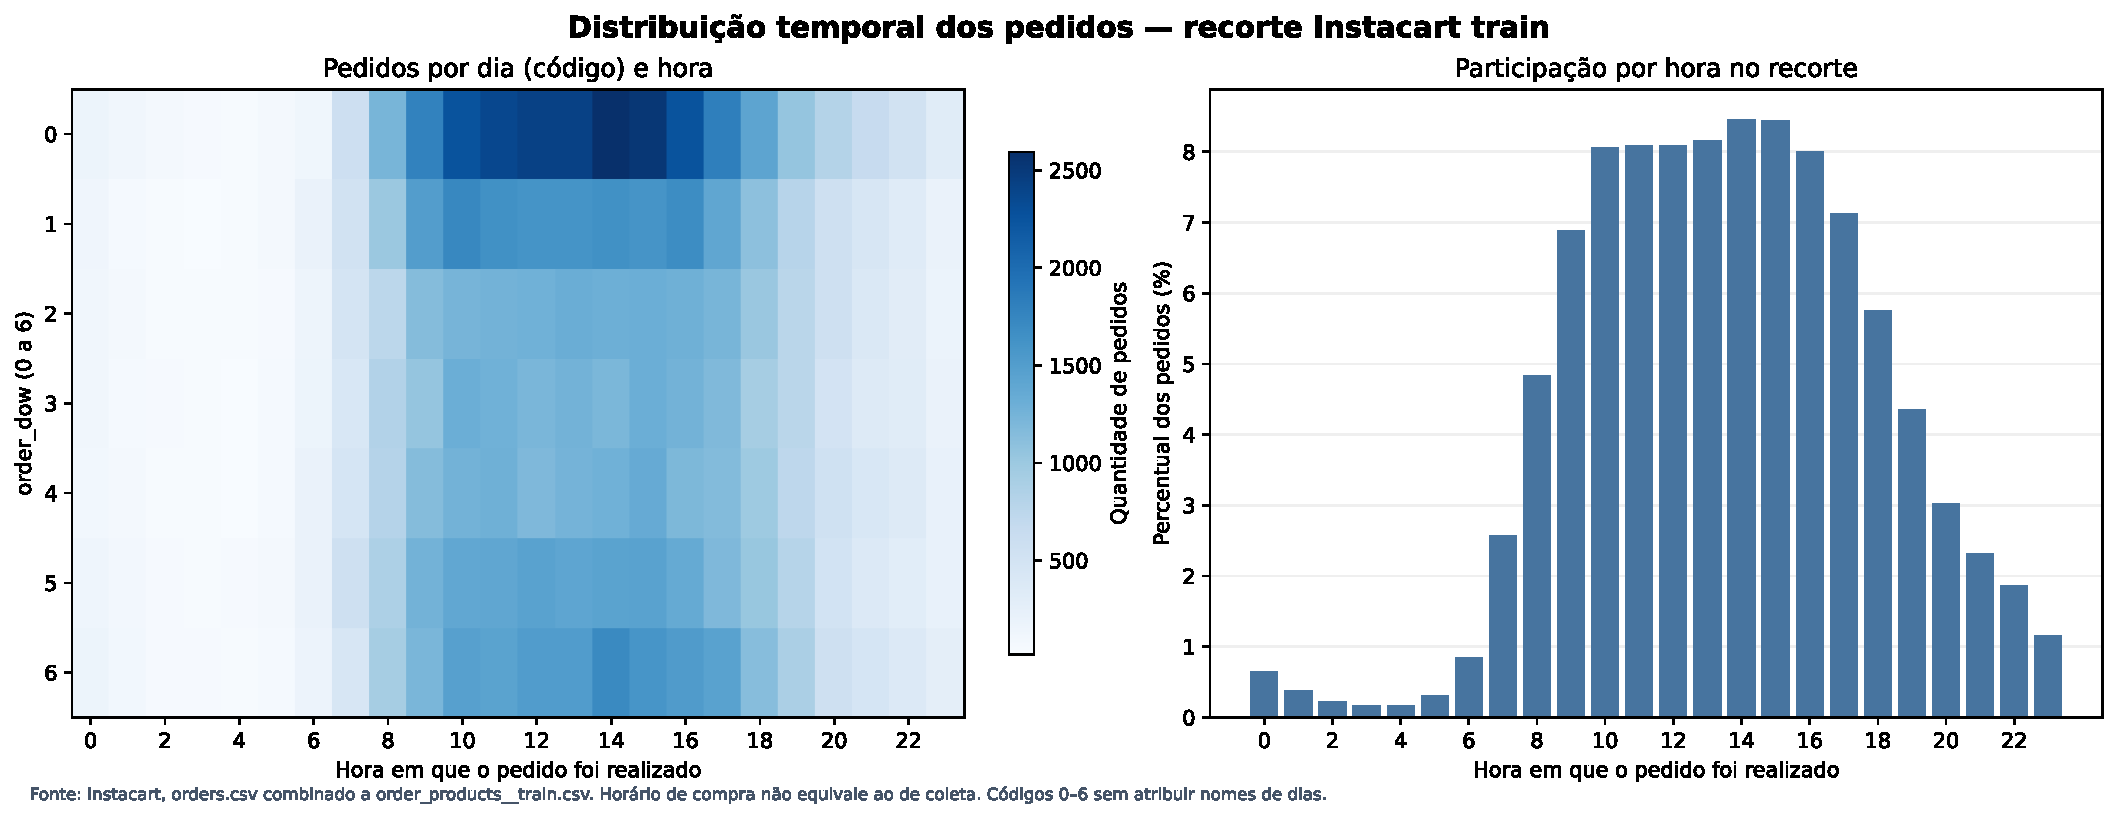
\includegraphics[width=\columnwidth]{figs/padroes_temporais.pdf}
\caption{Distribuição dos 131.209 pedidos do conjunto \textit{train} do Instacart por código do dia da semana (0 a 6) e horário de realização da compra, evidenciando os períodos de maior concentração de pedidos.}
\label{fig:temporal}
\end{figure}

Conforme a Figura~\ref{fig:temporal}, a maior concentração de pedidos ocorreu às 14h, com 11.103 pedidos, e no dia de código 0, com 27.465 registros. Esses horários correspondem à realização das compras, não necessariamente à coleta dos produtos.

Os resultados possuem limitações. O layout é hipotético e não considera corredores, obstáculos, congestionamentos ou a localização individual dos produtos; as distâncias são medidas em passos; os tempos de coleta e a capacidade por turno são estimativas baseadas em hipóteses operacionais, e não medições reais; o Modelo 1 foi avaliado nos 10.000 primeiros pedidos do recorte; e os dados provêm de uma operação de outro país. Essa ausência de corredores decorre de o Instacart não fornecer a planta da loja; com corredores, bastaria trocar a métrica de Manhattan pelas menores distâncias no grafo da loja (por exemplo, via Dijkstra), sem alterar os algoritmos. A aplicação dos métodos em supermercados físicos exigiria validar essas condições com dados e plantas reais.
